\documentclass{article}
\PassOptionsToPackage{numbers,compress}{natbib}
\usepackage[preprint]{neurips_2026}
\usepackage[utf8]{inputenc}
\usepackage[T1]{fontenc}
\usepackage{amsmath,amsfonts,graphicx,booktabs,microtype}
\usepackage[hidelinks]{hyperref}
\usepackage{url}
% Generated only from immutable measured artifacts; comparison SHA256 88daaa54bb2ff72a584d23cdd7cbf68ebc2339f33e8c579379ac8db945074777
% Qualitative review SHA256 feabf05a5c893e8a85adc8fd95415a4b72445ac5e56e7bffb5d198ccc98c657d
\newcommand{\WinnerFamily}{A1}
\newcommand{\WinnerEpoch}{300}
\newcommand{\WinnerVariant}{EMA}
\newcommand{\WinnerSeed}{123}
\newcommand{\WinnerSchedule}{paired linear decay after 200}
\newcommand{\WinnerSettings}{G64/D64, G/D rates 0.0002/0.0002}
\newcommand{\WinnerDetails}{real-image horizontal flips}
\newcommand{\WinnerValPair}{37.89, 36.94; 37.41}
\newcommand{\ControlValPair}{43.70, 44.84; 44.27}
\newcommand{\WinnerEpochMode}{300/EMA}
\newcommand{\ControlEpochMode}{250/EMA}
\newcommand{\WinnerTestFID}{37.50}
\newcommand{\ControlTestFID}{44.61}
\newcommand{\OriginalTestFID}{45.28}
\newcommand{\WinnerTestIS}{5.17}
\newcommand{\ControlTestIS}{5.04}
\newcommand{\OriginalTestIS}{4.70}
\newcommand{\TestDifference}{7.78}
\newcommand{\TestDirection}{lower}
\newcommand{\PairDifferenceOneTwoThree}{-5.81}
\newcommand{\PairDifferenceThreeOneFour}{-7.90}
\newcommand{\RzeroBest}{315.44}
\newcommand{\TotalRuns}{43}
\newcommand{\SelectedHash}{abeb5ba50f41}
\newcommand{\SettledNodeHours}{5.64}
\newcommand{\OriginalValFID}{45.94}
\newcommand{\RealRealFID}{14.51}
\newcommand{\VisualFinding}{Generated grids show varied palettes and coarse portrait, landscape and architectural motifs. Faces, hands and object boundaries remain distorted; the lower FID does not establish consistently coherent paintings.}
\newcommand{\FailureFinding}{Its fixed grid is nearly gray and low contrast, with faint varying structures rather than literally identical outputs.}

\title{Painting Generation with a Deep Convolutional GAN}
\author{Ricardo Silva Buarque\\ECE285: Deep Generative Models, UC San Diego}
\begin{document}
\maketitle
\begin{abstract}
An unconditional deep convolutional GAN is trained on WikiArt paintings.
A controlled, single-seed learning-rate comparison selects epoch \SelectedEpoch.
Final held-out probability-feature FID is \FinalFID\ and aggregate Inception
Score (IS) is \FinalIS\ over \FinalCount\ images. Fresh draws exhibit varied
palettes and painterly structures, with coarse or distorted details.
\end{abstract}

\section{Data, model, and training}
Kaggle's \texttt{steubk/wikiart}, version 1, supplies 81,444 decoded paintings
with zero decode failures. The first 64 bits of SHA256(42:SHA256(file bytes)),
divided by $2^{64}$, assign train below 0.8, validation below 0.9, and test
otherwise: 65,089/8,155/8,200 images. Identical-byte copies (80,716 unique
hashes) share a fold and are retained. Artist independence and near-duplicate
separation are not established. Images become RGB, are bilinearly resized to
shorter edge 64, center-cropped to $64\times64$, and scaled to $[-1,1]$.
Resizing preserves aspect ratio; cropping removes edge content.

The DCGAN architecture\citep{radford,pytorch} maps $z\sim\mathcal N(0,I_{100})$
through transposed-convolution channels $512,256,128,64,3$, with BatchNorm/ReLU
in hidden blocks and final tanh. Spatial sizes are $4,8,16,32,64$.
D uses channels $64,128,256,512,1$, stride-two downsampling, LeakyReLU(0.2),
BatchNorm in the three middle blocks, and one scalar logit $s(x)$.
G/D contain 3,576,704/2,765,568 parameters. Writing $D(x)=\sigma(s(x))$,
the discriminator and non-saturating generator objectives\citep{goodfellow} are
\begin{align}
L_D&=-\mathbb E_x\log D(x)-\mathbb E_z\log[1-D(G(z))],\nonumber\\
L_G&=-\mathbb E_z\log D(G(z)).
\end{align}
D takes one update using detached fakes; G then uses a fresh D forward.
Fused logit BCE estimates each expectation by its minibatch mean; D's loss
sums two means. D parameters are frozen during G's step, while its train-mode
BatchNorm buffers update. Preview/evaluation uses G in evaluation mode.

Adam uses betas $(0.5,0.999)$\citep{pytorch}, batch 128 and training seed 42.
Conv weights start as $\mathcal N(0,0.02^2)$; BatchNorm scales as
$\mathcal N(1,0.02^2)$, biases zero. Two arms compare common G/D rates
$2\times10^{-4}$ and $10^{-4}$, with all other settings fixed and 100 epochs
each. Both resume at $2\to50\to100$ epochs, matching loader-worker lifecycles.
The smaller step tests possible stabilization versus slower learning, without
isolating G/D rate effects. The 200 epochs take 1,264.3 training seconds and
101,800 D/G update pairs; validation and allocation overhead are separate.

\begin{figure}[ht!]
\centering
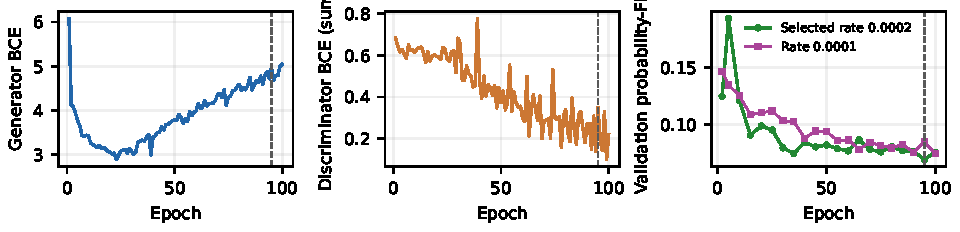
\includegraphics[width=\linewidth]{figures/training_diagnostics.pdf}
\caption{Measured minibatch-averaged G/D objectives for the selected-rate arm,
and validation probability-FID for both rates. Dashed lines mark selected
epoch 95. Losses oscillate and do not establish game convergence.}
\label{fig:history}
\end{figure}

\section{Selection, generated paintings, and limitations}
Validation uses 1,024 fixed references and seed-43 priors at epoch 2 and
every five epochs. Global minimum probability-FID selects across arms;
ties prefer baseline, then earlier epoch.

\begin{figure}[ht!]
\centering
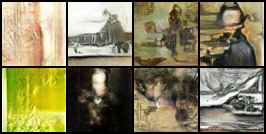
\includegraphics[width=0.52\linewidth]{figures/prior_samples_report.png}
\caption{First eight fresh standard-normal draws (seed 45), epoch 95.
Fixed intensity mapping; no image selection or input painting.}
\label{fig:samples}
\end{figure}

The choice was frozen at 08:27:26 UTC, 12 November 2026, before test evaluation.
Only the selected model is tested: \FinalCount\ references, prior seed 144,
reference-selection seed 100144. Separate seeds avoid training's prior seed 44.

The assigned Ignite protocol\citep{ignite} uses frozen torchvision Inception-v3
\texttt{IMAGENET1K\_V1}. Both real/generated RGB tensors map to $[0,1]$, then
antialiased bilinear $299\times299$ resize and ImageNet mean/std normalization;
\texttt{transform\_input=True} is retained. FID uses \emph{1,000 class probabilities},
not standard 2,048 pooled features. IS is aggregate, without split averaging.
All final outputs use checkpoint SHA256 prefix \CheckpointShortHash.

\begin{center}
\begin{tabular}{lccc}
\toprule
Rate / evaluation & Best epoch & Probability-FID & Aggregate IS \\
\midrule
$2\times10^{-4}$, validation ($N=1024$) & \BaselineEpoch & \BaselineFID & \BaselineIS \\
$10^{-4}$, validation ($N=1024$) & \LowerRateEpoch & \LowerRateFID & \LowerRateIS \\
Selected, test ($N=\FinalCount$) & \SelectedEpoch & \FinalFID & \FinalIS \\
\bottomrule
\end{tabular}
\end{center}

The baseline wins the declared FID criterion despite lower IS. This one-seed,
finite-validation ranking is not a population or perceptual optimum.
Different validation/test references and counts prevent attributing their score
difference to training improvement. ImageNet scores do not establish artistic
quality, coverage, or originality. Probability vectors sum to one, so covariance
rank is at most 999; finite-sample estimation and repeated checkpoint selection
remain limitations. Independent training seeds and an artist/near-duplicate-aware
split would test ranking robustness and generalization.

Code, weights, and figure regeneration:
\url{https://github.com/rsilvabuarque/ECE285_HW2_RSB}.

{\small
\begin{thebibliography}{4}
\bibitem{goodfellow} I. J. Goodfellow et al. Generative Adversarial Nets.
NeurIPS, 2014. \href{https://arxiv.org/abs/1406.2661}{arXiv:1406.2661}.
\bibitem{radford} A. Radford, L. Metz, and S. Chintala. Unsupervised
Representation Learning with Deep Convolutional Generative Adversarial Networks.
ICLR, 2016. \href{https://arxiv.org/abs/1511.06434}{arXiv:1511.06434}.
\bibitem{pytorch} PyTorch. \href{https://pytorch.org/tutorials/beginner/dcgan_faces_tutorial.html}{DCGAN Tutorial} (architecture and Adam recipe).
\bibitem{ignite} PyTorch-Ignite. \href{https://pytorch-ignite.ai/blog/gan-evaluation-with-fid-and-is/}{GAN evaluation using FID and IS}.
\end{thebibliography}
}
\end{document}
